% STATUS: ACTIVE -- first-order gain model, lambda_f = 1: Kalman filter on a_x step by step, observability matrix, and the link.
% ======================================================
% Compile: xelatex 0927_obs_first_order.tex   (from reference/eq17_analysis/derivation/)
% Notation: 0921_5state_noap_simple.tex (teacher chain) with delta a removed; Kalman filter = Meng dissertation (4.12)-(4.15)
%           with lambda_f = 1, gain written L (entries ell_ij) as in the teacher's closed-loop estimator.
% Equations only; the reading is done in conversation (derivation-workflow rule 10).
% Figures: fig_noap_first_order_is_average.png (plot_5state_noap_first_order_is_average.m),
%          fig_noap_weight_per_height.png       (plot_5state_noap_weight_per_height.m)
% Runs:    test_results/temp_5state_noap/ladder_ramp16_Td{5,15}_lf1_o1.mat (plane, 5 seeds)
% ======================================================
\documentclass[11pt,a4paper]{ctexart}
\usepackage[fleqn]{amsmath}
\usepackage{amssymb,bm}
\setlength{\mathindent}{0pt}
\usepackage{geometry}
\geometry{margin=2.0cm}
\usepackage{graphicx}
\graphicspath{{figures/}}
\setlength{\parindent}{0pt}
\setlength{\parskip}{0.3em}
\setlength{\abovedisplayskip}{4pt}
\setlength{\belowdisplayskip}{4pt}
\newcommand{\lc}{\lambda_c}
\newcommand{\hd}[1]{\par\medskip\noindent\underline{\textbf{#1}}\par\nobreak\vspace{0.2ex}}
\pagestyle{plain}

\begin{document}

\begin{center}\textbf{\large First-order gain model, $\lambda_f = 1$: Kalman filter, observability matrix, and the link}\end{center}

%======================================================================
\section{Model}

\hd{Motion error (from 0921, $\delta a_x$ removed)}
\[
\delta x[k+1] = \lc \cdot \delta x[k] - F_{dx}[k]\cdot e_{a_x}[k] - \varepsilon[k], \qquad
F_{dx}[k] = f_{dx}[k] + (1-\lc)\textstyle\sum_{i=1}^{d} f_{dx}[k-i]
\]

\hd{Parameter model, estimator, error}
\[
a_x[k+1] = a_x[k], \qquad \hat a_x[k+1] = \hat a_x[k], \qquad e_{a_x}[k] = a_x[k] - \hat a_x[k], \qquad e_{a_x}[k+1] = e_{a_x}[k]
\]

\hd{State equation}
\[
\begin{aligned}
\delta x_1[k+1] &= \delta x_2[k] \\
\delta x_2[k+1] &= \delta x_3[k] \\
\delta x_3[k+1] &= \lc \cdot \delta x_3[k] - F_{dx}[k]\cdot e_{a_x}[k] - \varepsilon[k] \\
a_x[k+1] &= a_x[k]
\end{aligned}
\]

\hd{Output equation}
\[
\begin{aligned}
y_1[k] &= \delta x_m[k] = \delta x_1[k] + n_x[k] \\
y_2[k] &= a_{xm}[k] = a_x[k] + n_a[k]
\end{aligned}
\]

\hd{Error model}
\[
\mathbf{e}[k] = \begin{bmatrix} e_{\delta x_1}[k] \\ e_{\delta x_2}[k] \\ e_{\delta x_3}[k] \\ e_{a_x}[k] \end{bmatrix}, \quad
\mathbf{F}_e[k] =
\begin{bmatrix}
0 & 1 & 0 & 0 \\
0 & 0 & 1 & 0 \\
0 & 0 & \lc & -F_{dx}[k] \\
0 & 0 & 0 & 1
\end{bmatrix}, \quad
\mathbf{H} =
\begin{bmatrix} \mathbf{H}_1 \\ \mathbf{H}_2 \end{bmatrix} =
\begin{bmatrix}
1 & 0 & 0 & 0 \\
0 & 0 & 0 & 1
\end{bmatrix}
\]
\[
\mathbf{Q} = \mathrm{diag}\big(0,\;0,\;Q_{33},\;0\big), \quad Q_{33} = \mathrm{Var}(\varepsilon), \qquad
\mathbf{R} = \mathrm{diag}\big(R_1,\;R_2\big), \quad R_1 = \mathrm{Var}(n_x),\; R_2 = \mathrm{Var}(n_a)
\]

%======================================================================
\section{Kalman filter}

\hd{Prediction}
\[
\begin{aligned}
\hat{\mathbf{x}}^f[k] &= \text{state equation applied to } \hat{\mathbf{x}}[k-1] \\
\mathbf{P}^f[k] &= \mathbf{F}_e[k-1]\,\mathbf{P}[k-1]\,\mathbf{F}_e^{\top}[k-1] + \mathbf{Q}
\end{aligned}
\]

\hd{Update}
\[
\begin{aligned}
\mathbf{L}[k] &= \mathbf{P}^f[k]\,\mathbf{H}^{\top}\big(\mathbf{H}\,\mathbf{P}^f[k]\,\mathbf{H}^{\top} + \mathbf{R}\big)^{-1} \\
\hat{\mathbf{x}}[k] &= \hat{\mathbf{x}}^f[k] + \mathbf{L}[k]\,\big(\mathbf{y}[k] - \mathbf{H}\,\hat{\mathbf{x}}^f[k]\big) \\
\mathbf{P}[k] &= \big(\mathbf{I} - \mathbf{L}[k]\,\mathbf{H}\big)\,\mathbf{P}^f[k]
\end{aligned}
\]

%======================================================================
\section{The $a_x$ element, $y_2$ only}

\hd{Prediction of $P_{aa}$}
\[
\begin{aligned}
\big(\mathbf{F}_e\,\mathbf{P}\,\mathbf{F}_e^{\top}\big)_{44} &= [\,0\;\;0\;\;0\;\;1\,]\;\mathbf{P}\;[\,0\;\;0\;\;0\;\;1\,]^{\top} = P_{aa} \\
P^f_{aa}[k] &= P_{aa}[k-1] + Q_{44} = P_{aa}[k-1]
\end{aligned}
\]

\hd{Gain}
\[
\begin{aligned}
\mathbf{H}_2\,\mathbf{P}^f\,\mathbf{H}_2^{\top} &= P^f_{aa} \\
\ell_{42}[k] &= \frac{P^f_{aa}[k]}{P^f_{aa}[k] + R_2}
\end{aligned}
\]

\hd{Update of $P_{aa}$}
\[
\begin{aligned}
P_{aa}[k] &= \big(1 - \ell_{42}[k]\big)\,P^f_{aa}[k] = \frac{R_2}{P^f_{aa}[k] + R_2}\,P^f_{aa}[k] \\
\frac{1}{P_{aa}[k]} &= \frac{P^f_{aa}[k] + R_2}{R_2\,P^f_{aa}[k]} = \frac{1}{P^f_{aa}[k]} + \frac{1}{R_2} = \frac{1}{P_{aa}[k-1]} + \frac{1}{R_2} \\
\frac{1}{P_{aa}[k]} &= \frac{1}{P_{aa}[0]} + \frac{k}{R_2}
\end{aligned}
\]

\hd{Gain written with $P_{aa}[k]$}
\[
\ell_{42}[k] = \frac{P^f_{aa}[k]}{P^f_{aa}[k] + R_2} = \frac{P_{aa}[k]}{R_2}
= \frac{1/R_2}{\dfrac{1}{P_{aa}[0]} + \dfrac{k}{R_2}}
\]

\hd{Update of $\hat a_x$}
\[
\hat a_x[k] = \hat a_x[k-1] + \ell_{42}[k]\,\big(y_2[k] - \hat a_x[k-1]\big)
\]

\hd{Closed form (induction)}
\[
\begin{aligned}
\text{claim:}\quad \hat a_x[k] &= \frac{\dfrac{1}{P_{aa}[0]}\,\hat a_x[0] + \dfrac{1}{R_2}\sum_{j=1}^{k} y_2[j]}{\dfrac{1}{P_{aa}[k]}} \\[0.8ex]
k \to k+1:\quad \hat a_x[k+1] &= \big(1 - \ell_{42}[k+1]\big)\,\hat a_x[k] + \ell_{42}[k+1]\,y_2[k+1] \\
&= \frac{P_{aa}[k+1]}{P_{aa}[k]}\,\hat a_x[k] + \frac{P_{aa}[k+1]}{R_2}\,y_2[k+1] \\
&= P_{aa}[k+1]\left(\frac{1}{P_{aa}[0]}\,\hat a_x[0] + \frac{1}{R_2}\sum_{j=1}^{k} y_2[j] + \frac{1}{R_2}\,y_2[k+1]\right)
\end{aligned}
\]
\[
\Big(\,1 - \ell_{42}[k+1] = \frac{R_2}{P_{aa}[k] + R_2} = \frac{P_{aa}[k+1]}{P_{aa}[k]}\,\Big)
\]

\hd{Substitute $y_2[j] = a_x[j] + n_a[j]$}
\[
\hat a_x[k] = \frac{\dfrac{1}{P_{aa}[0]}\,\hat a_x[0] + \dfrac{1}{R_2}\sum_{j=1}^{k} a_x[j]}{\dfrac{1}{P_{aa}[0]} + \dfrac{k}{R_2}}
\;+\; \frac{\dfrac{1}{R_2}\sum_{j=1}^{k} n_a[j]}{\dfrac{1}{P_{aa}[0]} + \dfrac{k}{R_2}}
\]

%======================================================================
\section{Observability matrix}

\hd{Definition (prediction only: $\mathbf{F}_e$, no $\mathbf{L}$, no noise)}
\[
\bm{\Phi}(k_0+j,\,k_0) = \mathbf{F}_e[k_0+j-1]\cdots\mathbf{F}_e[k_0], \qquad \bm{\Phi}(k_0,k_0) = \mathbf{I}, \qquad
\mathbf{O}(k_0) =
\begin{bmatrix}
\mathbf{H}\,\bm{\Phi}(k_0,k_0) \\ \mathbf{H}\,\bm{\Phi}(k_0+1,k_0) \\ \mathbf{H}\,\bm{\Phi}(k_0+2,k_0) \\ \vdots
\end{bmatrix}
\]

\hd{The $e_{a_x}$ column of $\bm{\Phi}$}
\[
\begin{aligned}
\bm{\phi}[j] &= \bm{\Phi}(k_0+j,k_0)\,[\,0\;\;0\;\;0\;\;1\,]^{\top} = \begin{bmatrix} \phi_1[j] & \phi_2[j] & \phi_3[j] & \phi_4[j] \end{bmatrix}^{\top} \\
\bm{\phi}[0] &= [\,0\;\;0\;\;0\;\;1\,]^{\top} \\
\bm{\phi}[j+1] &= \mathbf{F}_e[k_0+j]\,\bm{\phi}[j]
\end{aligned}
\]
\[
\begin{aligned}
\phi_1[j+1] &= \phi_2[j] \\
\phi_2[j+1] &= \phi_3[j] \\
\phi_3[j+1] &= \lc \cdot \phi_3[j] - F_{dx}[k_0+j]\cdot\phi_4[j] \\
\phi_4[j+1] &= \phi_4[j]
\end{aligned}
\]
\[
\begin{aligned}
\phi_4[j] &= 1 \\
\phi_3[j] &= -\textstyle\sum_{i=0}^{j-1} \lc^{\,j-1-i}\,F_{dx}[k_0+i] \\
\phi_2[j] &= \phi_3[j-1] \\
\phi_1[j] &= \phi_3[j-2]
\end{aligned}
\]

\hd{The $e_{a_x}$ column of $\mathbf{O}$}
\[
\begin{aligned}
\mathbf{H}_1\,\bm{\phi}[j] &= \phi_1[j] = -\textstyle\sum_{i=0}^{j-3} \lc^{\,j-3-i}\,F_{dx}[k_0+i] \quad (j \ge 3), \qquad \mathbf{H}_1\,\bm{\phi}[0] = \mathbf{H}_1\,\bm{\phi}[1] = \mathbf{H}_1\,\bm{\phi}[2] = 0 \\
\mathbf{H}_2\,\bm{\phi}[j] &= \phi_4[j] = 1
\end{aligned}
\]

\hd{Constant $F_{dx}$}
\[
\phi_3[j] = -F_{dx}\,\frac{1-\lc^{\,j}}{1-\lc} \;\xrightarrow{\;j \to \infty\;}\; -\frac{F_{dx}}{1-\lc}, \qquad
\mathbf{H}_1\,\bm{\phi}[j] \;\to\; -\frac{F_{dx}}{1-\lc}
\]

\hd{$F_{dx}$ at constant velocity (implementable control effort, $\delta x_m \approx 0$, $\hat a_x f_{dx}$ constant)}
\[
\begin{aligned}
\hat a_x f_{dx} &= \Delta x_d^{d} + (1-\lc)\big[\,0 - d\,\hat a_x f_{dx}\,\big], \qquad \Delta x_d^{d} = \big(1 + (1-\lc)d\big)\Delta x_d \\
\hat a_x f_{dx}\,\big(1 + (1-\lc)d\big) &= \big(1 + (1-\lc)d\big)\Delta x_d \;\;\Rightarrow\;\; f_{dx} = \frac{\Delta x_d}{\hat a_x} \\
F_{dx} &= f_{dx} + (1-\lc)\,d\,f_{dx} = \big(1 + (1-\lc)d\big)\,\frac{\Delta x_d}{\hat a_x}
\end{aligned}
\]

%======================================================================
\section{Link: $\mathbf{O}$ inside the Kalman filter}

\hd{$y_2$: the row of $\mathbf{O}$ is $\mathbf{H}_2$ itself ($\phi_4 = 1$)}
\[
\frac{1}{P_{aa}[k]} - \frac{1}{P_{aa}[k-1]} = \frac{1}{R_2} = \frac{\big(\mathbf{H}_2\,\bm{\phi}[j]\big)^2}{R_2}
\]

\hd{$y_1$: $\mathbf{H}_1$ has $0$ in the $a_x$ column; the path is built in $\mathbf{P}^f$}
\[
\begin{aligned}
P^f_{3a}[k] &= \big(\mathbf{F}_e\,\mathbf{P}\,\mathbf{F}_e^{\top}\big)_{34}
= [\,0\;\;0\;\;\lc\;\;-F_{dx}\,]\;\mathbf{P}\;[\,0\;\;0\;\;0\;\;1\,]^{\top} = \lc\,P_{3a}[k-1] - F_{dx}[k-1]\,P_{aa}[k-1] \\
P^f_{2a}[k] &= P_{3a}[k-1] \\
P^f_{1a}[k] &= P_{2a}[k-1]
\end{aligned}
\]
\[
\begin{aligned}
&\text{prediction only, } P_{3a}[k_0] = 0, \ P_{aa} \text{ constant over the window:} \\
&P_{3a}[k_0+j] = \phi_3[j]\,P_{aa}, \qquad P_{1a}[k_0+j] = \phi_1[j]\,P_{aa} = \big(\mathbf{H}_1\,\bm{\phi}[j]\big)\,P_{aa}
\end{aligned}
\]
\[
\ell_{41}[k] = \frac{P^f_{a1}[k]}{P^f_{11}[k] + R_1} \approx \frac{\big(\mathbf{H}_1\,\bm{\phi}[j]\big)\,P_{aa}}{P^f_{11}[k] + R_1}, \qquad
\frac{1}{P_{aa}[k]} - \frac{1}{P_{aa}[k-1]} \approx \frac{\big(\mathbf{H}_1\,\bm{\phi}[j]\big)^2}{P^f_{11}[k] + R_1}
\;\le\; \frac{\big(\mathbf{H}_1\,\bm{\phi}[j]\big)^2}{R_1}
\]

\hd{Both channels}
\[
\begin{aligned}
\frac{1}{P_{aa}[k]} &\approx \frac{1}{P_{aa}[0]} + \sum_{j=1}^{k}\big(w_2 + w_1[j]\big) \\
w_2 &= \frac{1}{R_2} \\
w_1[j] &= \frac{\big(\mathbf{H}_1\,\bm{\phi}[j]\big)^2}{P^f_{11}[j] + R_1} \approx \frac{1}{P^f_{11} + R_1}\left(\frac{1 + (1-\lc)d}{1-\lc}\,\frac{\Delta x_d[j]}{\hat a_x[j]}\right)^{2}
\end{aligned}
\]
\[
\hat a_x[k] \approx \frac{\dfrac{1}{P_{aa}[0]}\,\hat a_x[0] + \sum_{j=1}^{k}\big(w_2 + w_1[j]\big)\,a_x[j]}
{\dfrac{1}{P_{aa}[0]} + \sum_{j=1}^{k}\big(w_2 + w_1[j]\big)}
\]

%======================================================================
\section{Speed}

\[
\begin{aligned}
\Delta x_d &= \frac{(h_0 - h_b)\,R\,T_s}{T_d}, \qquad \text{steps per } R \text{ travelled} = \frac{T_d}{(h_0 - h_b)\,T_s} \\
\text{per } R \text{ travelled:}\quad & w_2\,\frac{T_d}{(h_0 - h_b)\,T_s} \;\propto\; T_d, \qquad
w_1\,\frac{T_d}{(h_0 - h_b)\,T_s} \;\propto\; \Delta x_d^{2}\,T_d \;\propto\; \frac{1}{T_d}
\end{aligned}
\]

\clearpage
\section*{Figure: $\hat a_x$ vs running average of $a_x$}
\begin{center}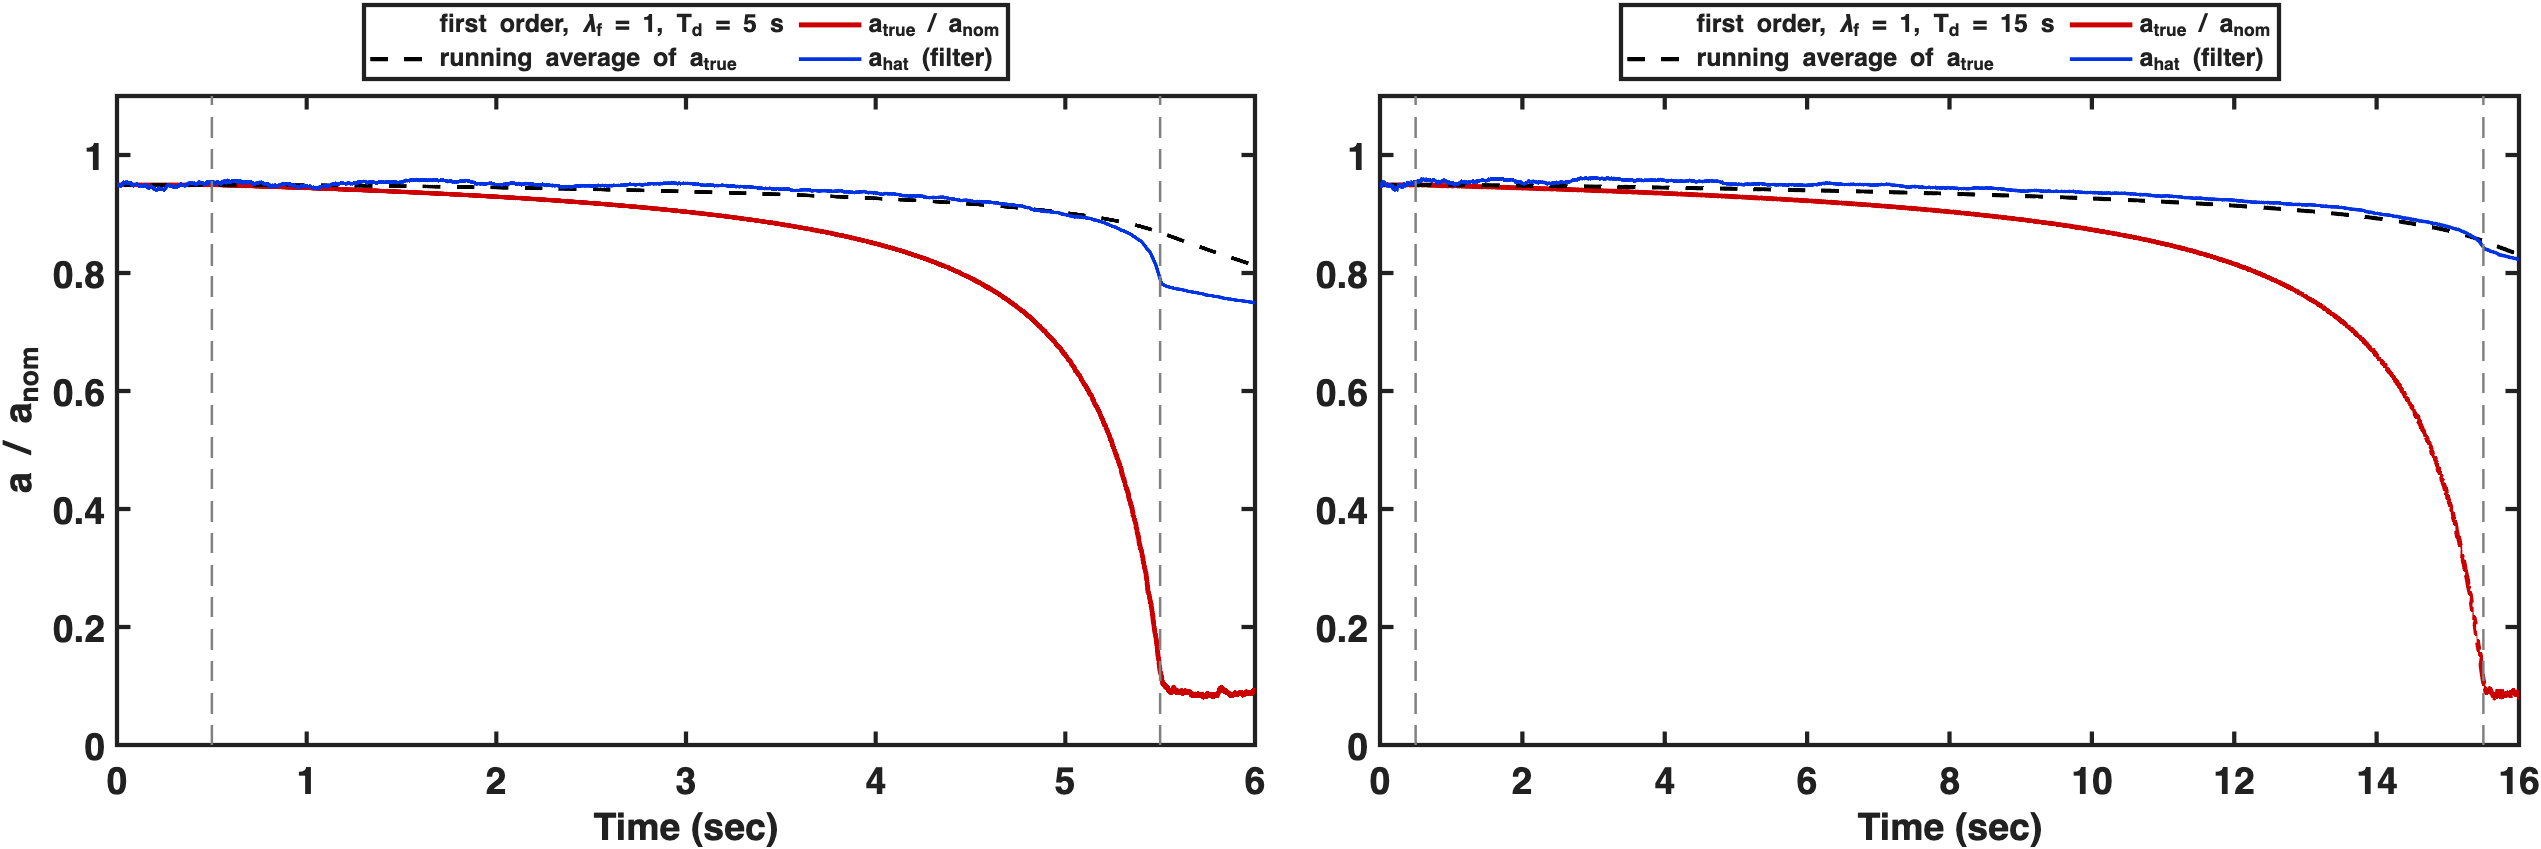
\includegraphics[width=\textwidth]{fig_noap_first_order_is_average.png}\end{center}

\section*{Figure: $1/P_{aa}$ added per step and per $R$ travelled}
\begin{center}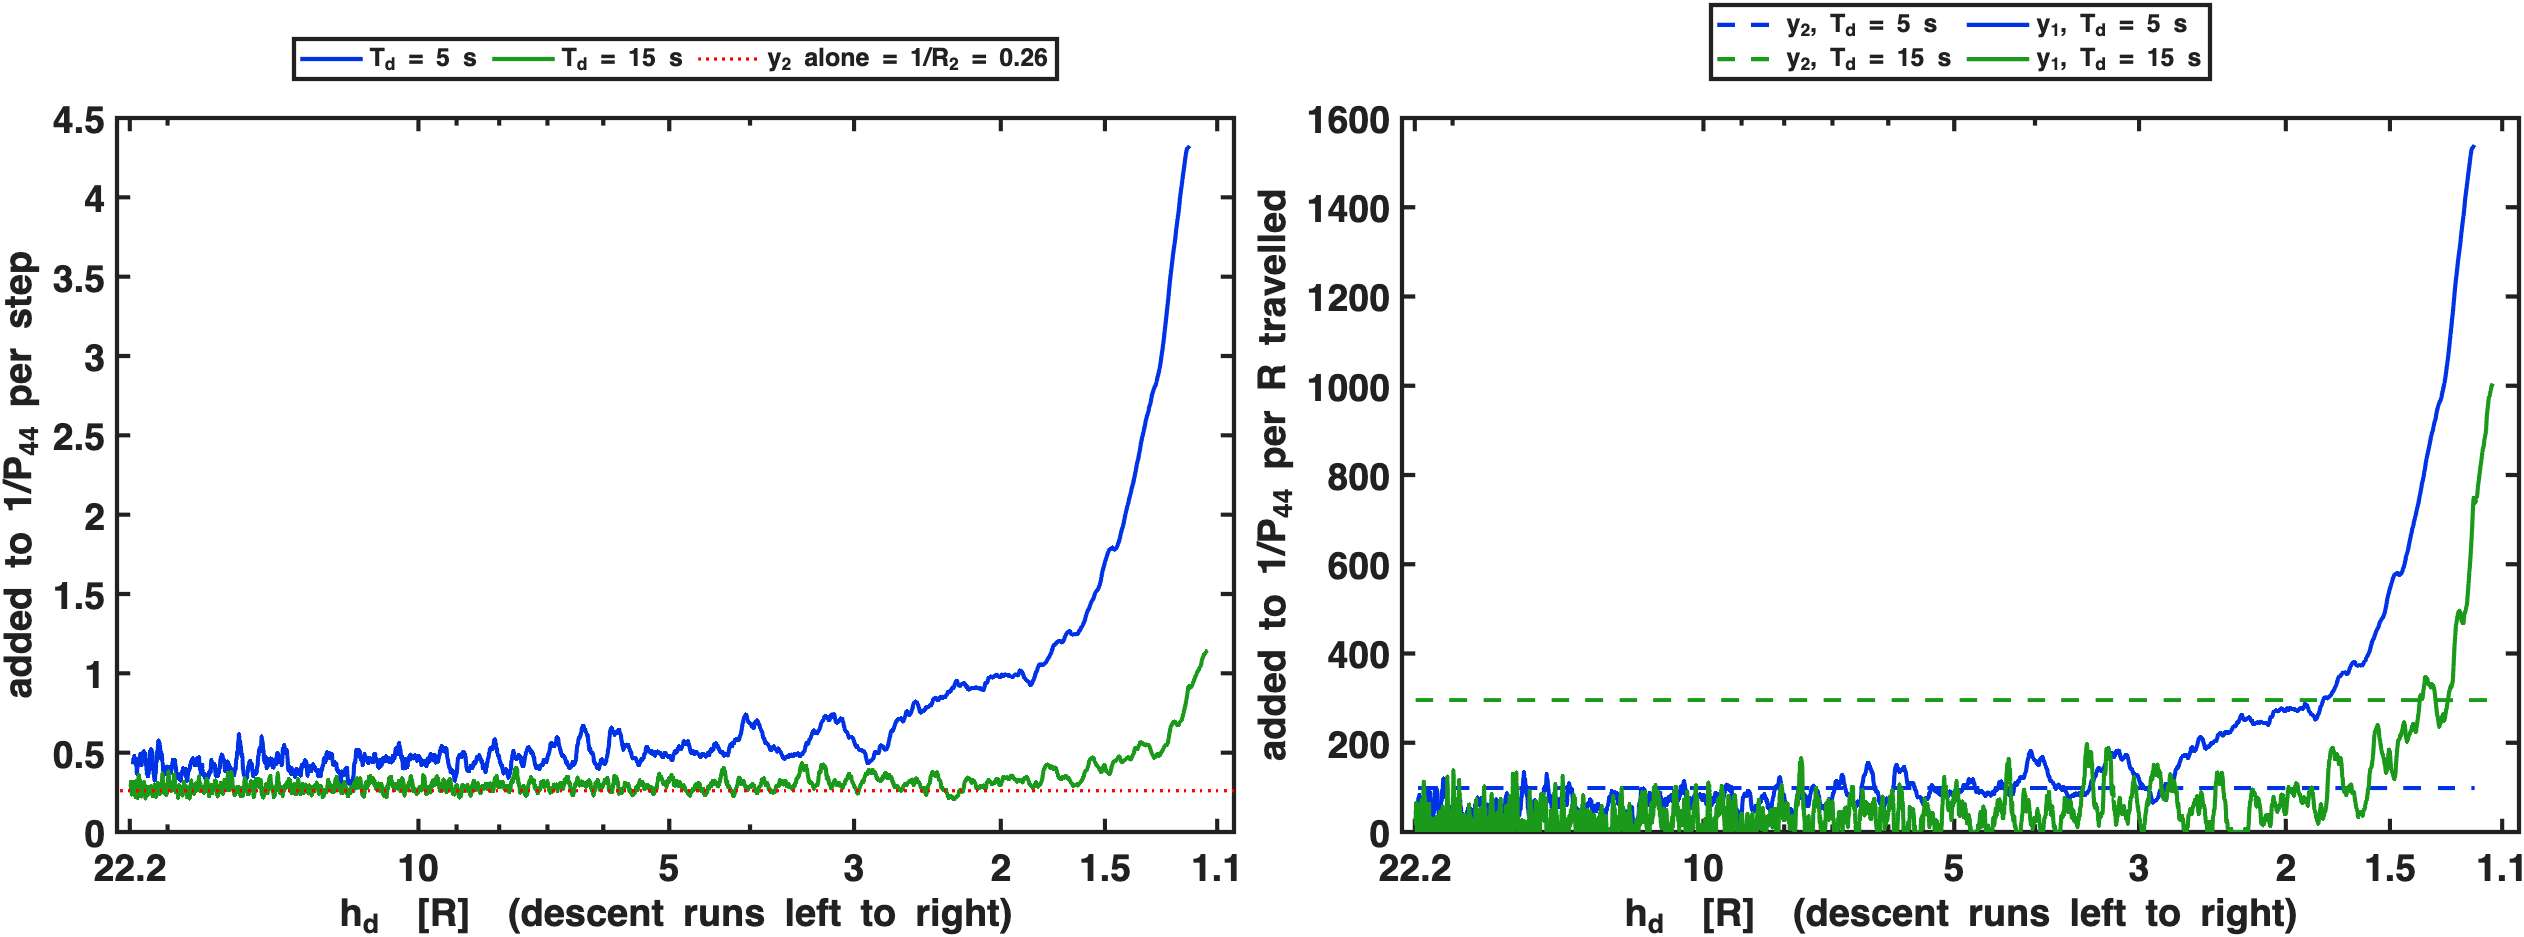
\includegraphics[width=\textwidth]{fig_noap_weight_per_height.png}\end{center}

\end{document}
